\tikzset{every picture/.style={line width=0.75pt}} %set default line width to 0.75pt        

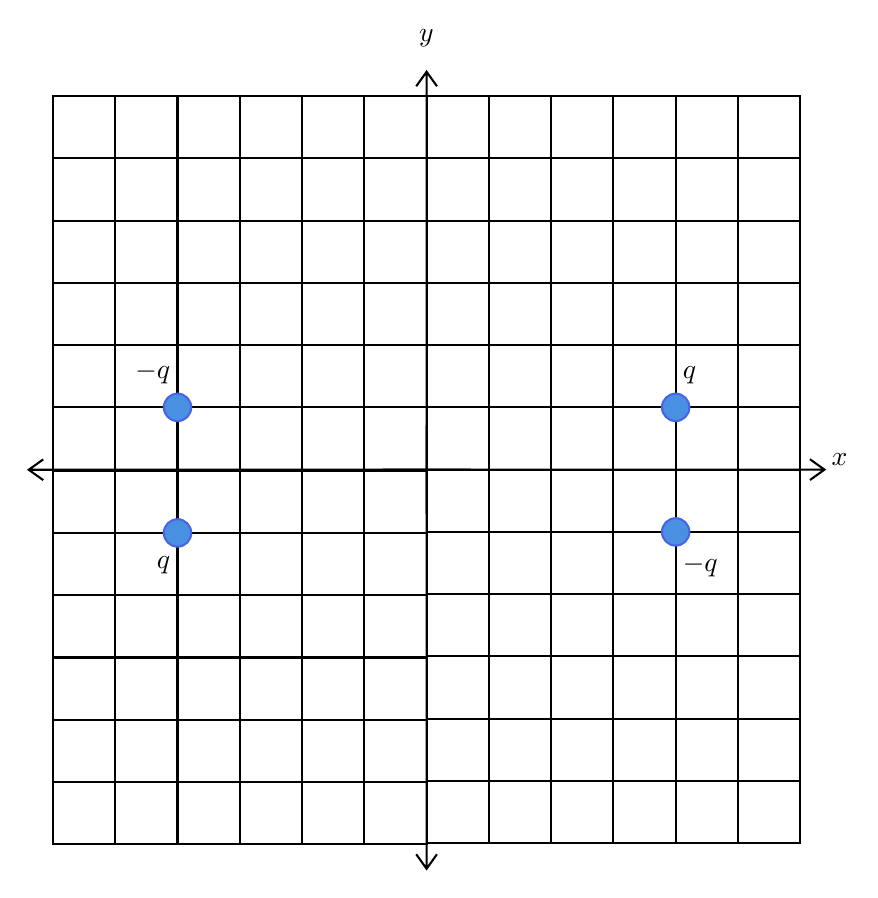
\begin{tikzpicture}[x=0.75pt,y=0.75pt,yscale=-1,xscale=1]
%uncomment if require: \path (0,657); %set diagram left start at 0, and has height of 657

%Shape: Axis 2D [id:dp1373512094917413] 
\draw  (259,275.7) -- (472,275.7)(280.3,84) -- (280.3,297) (465,270.7) -- (472,275.7) -- (465,280.7) (275.3,91) -- (280.3,84) -- (285.3,91)  ;
%Shape: Axis 2D [id:dp329188015017823] 
\draw  (301.6,275.76) -- (88.6,275.76)(280.3,468) -- (280.3,254.4) (95.6,280.76) -- (88.6,275.76) -- (95.6,270.76) (285.3,461) -- (280.3,468) -- (275.3,461)  ;
%Shape: Grid [id:dp7539739677566268] 
\draw  [draw opacity=0] (100.3,276.2) -- (280.3,276.2) -- (280.3,456.2) -- (100.3,456.2) -- cycle ; \draw   (130.3,276.2) -- (130.3,456.2)(160.3,276.2) -- (160.3,456.2)(190.3,276.2) -- (190.3,456.2)(220.3,276.2) -- (220.3,456.2)(250.3,276.2) -- (250.3,456.2) ; \draw   (100.3,306.2) -- (280.3,306.2)(100.3,336.2) -- (280.3,336.2)(100.3,366.2) -- (280.3,366.2)(100.3,396.2) -- (280.3,396.2)(100.3,426.2) -- (280.3,426.2) ; \draw   (100.3,276.2) -- (280.3,276.2) -- (280.3,456.2) -- (100.3,456.2) -- cycle ;
%Shape: Grid [id:dp2853097292529867] 
\draw  [draw opacity=0] (280.3,275.7) -- (460.3,275.7) -- (460.3,455.7) -- (280.3,455.7) -- cycle ; \draw   (310.3,275.7) -- (310.3,455.7)(340.3,275.7) -- (340.3,455.7)(370.3,275.7) -- (370.3,455.7)(400.3,275.7) -- (400.3,455.7)(430.3,275.7) -- (430.3,455.7) ; \draw   (280.3,305.7) -- (460.3,305.7)(280.3,335.7) -- (460.3,335.7)(280.3,365.7) -- (460.3,365.7)(280.3,395.7) -- (460.3,395.7)(280.3,425.7) -- (460.3,425.7) ; \draw   (280.3,275.7) -- (460.3,275.7) -- (460.3,455.7) -- (280.3,455.7) -- cycle ;
%Shape: Grid [id:dp3861257807049996] 
\draw  [draw opacity=0] (280.3,95.7) -- (460.3,95.7) -- (460.3,275.7) -- (280.3,275.7) -- cycle ; \draw   (310.3,95.7) -- (310.3,275.7)(340.3,95.7) -- (340.3,275.7)(370.3,95.7) -- (370.3,275.7)(400.3,95.7) -- (400.3,275.7)(430.3,95.7) -- (430.3,275.7) ; \draw   (280.3,125.7) -- (460.3,125.7)(280.3,155.7) -- (460.3,155.7)(280.3,185.7) -- (460.3,185.7)(280.3,215.7) -- (460.3,215.7)(280.3,245.7) -- (460.3,245.7) ; \draw   (280.3,95.7) -- (460.3,95.7) -- (460.3,275.7) -- (280.3,275.7) -- cycle ;
%Shape: Grid [id:dp2044452336417133] 
\draw  [draw opacity=0] (100.3,95.7) -- (280.3,95.7) -- (280.3,275.7) -- (100.3,275.7) -- cycle ; \draw   (130.3,95.7) -- (130.3,275.7)(160.3,95.7) -- (160.3,275.7)(190.3,95.7) -- (190.3,275.7)(220.3,95.7) -- (220.3,275.7)(250.3,95.7) -- (250.3,275.7) ; \draw   (100.3,125.7) -- (280.3,125.7)(100.3,155.7) -- (280.3,155.7)(100.3,185.7) -- (280.3,185.7)(100.3,215.7) -- (280.3,215.7)(100.3,245.7) -- (280.3,245.7) ; \draw   (100.3,95.7) -- (280.3,95.7) -- (280.3,275.7) -- (100.3,275.7) -- cycle ;
%Shape: Circle [id:dp6814120704702491] 
\draw  [color={rgb, 255:red, 74; green, 99; blue, 226 }  ,draw opacity=1 ][fill={rgb, 255:red, 74; green, 144; blue, 226 }  ,fill opacity=1 ] (393.7,245.7) .. controls (393.7,242.05) and (396.65,239.1) .. (400.3,239.1) .. controls (403.95,239.1) and (406.9,242.05) .. (406.9,245.7) .. controls (406.9,249.35) and (403.95,252.3) .. (400.3,252.3) .. controls (396.65,252.3) and (393.7,249.35) .. (393.7,245.7) -- cycle ;
%Shape: Circle [id:dp37300952646152163] 
\draw  [color={rgb, 255:red, 74; green, 99; blue, 226 }  ,draw opacity=1 ][fill={rgb, 255:red, 74; green, 144; blue, 226 }  ,fill opacity=1 ] (393.7,305.7) .. controls (393.7,302.05) and (396.65,299.1) .. (400.3,299.1) .. controls (403.95,299.1) and (406.9,302.05) .. (406.9,305.7) .. controls (406.9,309.35) and (403.95,312.3) .. (400.3,312.3) .. controls (396.65,312.3) and (393.7,309.35) .. (393.7,305.7) -- cycle ;
%Shape: Circle [id:dp5860262256290361] 
\draw  [color={rgb, 255:red, 74; green, 99; blue, 226 }  ,draw opacity=1 ][fill={rgb, 255:red, 74; green, 144; blue, 226 }  ,fill opacity=1 ] (153.7,306.2) .. controls (153.7,302.55) and (156.65,299.6) .. (160.3,299.6) .. controls (163.95,299.6) and (166.9,302.55) .. (166.9,306.2) .. controls (166.9,309.85) and (163.95,312.8) .. (160.3,312.8) .. controls (156.65,312.8) and (153.7,309.85) .. (153.7,306.2) -- cycle ;
%Shape: Circle [id:dp11907902437511675] 
\draw  [color={rgb, 255:red, 74; green, 99; blue, 226 }  ,draw opacity=1 ][fill={rgb, 255:red, 74; green, 144; blue, 226 }  ,fill opacity=1 ] (153.7,245.7) .. controls (153.7,242.05) and (156.65,239.1) .. (160.3,239.1) .. controls (163.95,239.1) and (166.9,242.05) .. (166.9,245.7) .. controls (166.9,249.35) and (163.95,252.3) .. (160.3,252.3) .. controls (156.65,252.3) and (153.7,249.35) .. (153.7,245.7) -- cycle ;

% Text Node
\draw (474,266.4) node [anchor=north west][inner sep=0.75pt]    {$x$};
% Text Node
\draw (280.22,73.6) node [anchor=south] [inner sep=0.75pt]    {$y$};
% Text Node
\draw (402.3,235.7) node [anchor=south west] [inner sep=0.75pt]    {$q$};
% Text Node
\draw (402.3,315.7) node [anchor=north west][inner sep=0.75pt]    {$-q$};
% Text Node
\draw (158.3,316.2) node [anchor=north east] [inner sep=0.75pt]    {$q$};
% Text Node
\draw (158.3,235.7) node [anchor=south east] [inner sep=0.75pt]    {$-q$};


\end{tikzpicture}
